% Options for packages loaded elsewhere
\PassOptionsToPackage{unicode}{hyperref}
\PassOptionsToPackage{hyphens}{url}
%
\documentclass[
  english,
  man]{apa6}
\usepackage{amsmath,amssymb}
\usepackage{lmodern}
\usepackage{ifxetex,ifluatex}
\ifnum 0\ifxetex 1\fi\ifluatex 1\fi=0 % if pdftex
  \usepackage[T1]{fontenc}
  \usepackage[utf8]{inputenc}
  \usepackage{textcomp} % provide euro and other symbols
\else % if luatex or xetex
  \usepackage{unicode-math}
  \defaultfontfeatures{Scale=MatchLowercase}
  \defaultfontfeatures[\rmfamily]{Ligatures=TeX,Scale=1}
\fi
% Use upquote if available, for straight quotes in verbatim environments
\IfFileExists{upquote.sty}{\usepackage{upquote}}{}
\IfFileExists{microtype.sty}{% use microtype if available
  \usepackage[]{microtype}
  \UseMicrotypeSet[protrusion]{basicmath} % disable protrusion for tt fonts
}{}
\makeatletter
\@ifundefined{KOMAClassName}{% if non-KOMA class
  \IfFileExists{parskip.sty}{%
    \usepackage{parskip}
  }{% else
    \setlength{\parindent}{0pt}
    \setlength{\parskip}{6pt plus 2pt minus 1pt}}
}{% if KOMA class
  \KOMAoptions{parskip=half}}
\makeatother
\usepackage{xcolor}
\IfFileExists{xurl.sty}{\usepackage{xurl}}{} % add URL line breaks if available
\IfFileExists{bookmark.sty}{\usepackage{bookmark}}{\usepackage{hyperref}}
\hypersetup{
  pdftitle={Battleships, exp. 1: intermediate results},
  pdfauthor={First Author1 \& Ernst-August Doelle1,2},
  pdflang={en-EN},
  pdfkeywords={keywords},
  hidelinks,
  pdfcreator={LaTeX via pandoc}}
\urlstyle{same} % disable monospaced font for URLs
\usepackage{graphicx}
\makeatletter
\def\maxwidth{\ifdim\Gin@nat@width>\linewidth\linewidth\else\Gin@nat@width\fi}
\def\maxheight{\ifdim\Gin@nat@height>\textheight\textheight\else\Gin@nat@height\fi}
\makeatother
% Scale images if necessary, so that they will not overflow the page
% margins by default, and it is still possible to overwrite the defaults
% using explicit options in \includegraphics[width, height, ...]{}
\setkeys{Gin}{width=\maxwidth,height=\maxheight,keepaspectratio}
% Set default figure placement to htbp
\makeatletter
\def\fps@figure{htbp}
\makeatother
\setlength{\emergencystretch}{3em} % prevent overfull lines
\providecommand{\tightlist}{%
  \setlength{\itemsep}{0pt}\setlength{\parskip}{0pt}}
\setcounter{secnumdepth}{-\maxdimen} % remove section numbering
% Make \paragraph and \subparagraph free-standing
\ifx\paragraph\undefined\else
  \let\oldparagraph\paragraph
  \renewcommand{\paragraph}[1]{\oldparagraph{#1}\mbox{}}
\fi
\ifx\subparagraph\undefined\else
  \let\oldsubparagraph\subparagraph
  \renewcommand{\subparagraph}[1]{\oldsubparagraph{#1}\mbox{}}
\fi
% Manuscript styling
\usepackage{upgreek}
\captionsetup{font=singlespacing,justification=justified}

% Table formatting
\usepackage{longtable}
\usepackage{lscape}
% \usepackage[counterclockwise]{rotating}   % Landscape page setup for large tables
\usepackage{multirow}		% Table styling
\usepackage{tabularx}		% Control Column width
\usepackage[flushleft]{threeparttable}	% Allows for three part tables with a specified notes section
\usepackage{threeparttablex}            % Lets threeparttable work with longtable

% Create new environments so endfloat can handle them
% \newenvironment{ltable}
%   {\begin{landscape}\centering\begin{threeparttable}}
%   {\end{threeparttable}\end{landscape}}
\newenvironment{lltable}{\begin{landscape}\centering\begin{ThreePartTable}}{\end{ThreePartTable}\end{landscape}}

% Enables adjusting longtable caption width to table width
% Solution found at http://golatex.de/longtable-mit-caption-so-breit-wie-die-tabelle-t15767.html
\makeatletter
\newcommand\LastLTentrywidth{1em}
\newlength\longtablewidth
\setlength{\longtablewidth}{1in}
\newcommand{\getlongtablewidth}{\begingroup \ifcsname LT@\roman{LT@tables}\endcsname \global\longtablewidth=0pt \renewcommand{\LT@entry}[2]{\global\advance\longtablewidth by ##2\relax\gdef\LastLTentrywidth{##2}}\@nameuse{LT@\roman{LT@tables}} \fi \endgroup}

% \setlength{\parindent}{0.5in}
% \setlength{\parskip}{0pt plus 0pt minus 0pt}

% \usepackage{etoolbox}
\makeatletter
\patchcmd{\HyOrg@maketitle}
  {\section{\normalfont\normalsize\abstractname}}
  {\section*{\normalfont\normalsize\abstractname}}
  {}{\typeout{Failed to patch abstract.}}
\patchcmd{\HyOrg@maketitle}
  {\section{\protect\normalfont{\@title}}}
  {\section*{\protect\normalfont{\@title}}}
  {}{\typeout{Failed to patch title.}}
\makeatother
\shorttitle{Battleships}
\keywords{keywords\newline\indent Word count: X}
\DeclareDelayedFloatFlavor{ThreePartTable}{table}
\DeclareDelayedFloatFlavor{lltable}{table}
\DeclareDelayedFloatFlavor*{longtable}{table}
\makeatletter
\renewcommand{\efloat@iwrite}[1]{\immediate\expandafter\protected@write\csname efloat@post#1\endcsname{}}
\makeatother
\usepackage{lineno}

\linenumbers
\usepackage{csquotes}
\ifxetex
  % Load polyglossia as late as possible: uses bidi with RTL langages (e.g. Hebrew, Arabic)
  \usepackage{polyglossia}
  \setmainlanguage[]{english}
\else
  \usepackage[main=english]{babel}
% get rid of language-specific shorthands (see #6817):
\let\LanguageShortHands\languageshorthands
\def\languageshorthands#1{}
\fi
\ifluatex
  \usepackage{selnolig}  % disable illegal ligatures
\fi
\newlength{\cslhangindent}
\setlength{\cslhangindent}{1.5em}
\newlength{\csllabelwidth}
\setlength{\csllabelwidth}{3em}
\newenvironment{CSLReferences}[2] % #1 hanging-ident, #2 entry spacing
 {% don't indent paragraphs
  \setlength{\parindent}{0pt}
  % turn on hanging indent if param 1 is 1
  \ifodd #1 \everypar{\setlength{\hangindent}{\cslhangindent}}\ignorespaces\fi
  % set entry spacing
  \ifnum #2 > 0
  \setlength{\parskip}{#2\baselineskip}
  \fi
 }%
 {}
\usepackage{calc}
\newcommand{\CSLBlock}[1]{#1\hfill\break}
\newcommand{\CSLLeftMargin}[1]{\parbox[t]{\csllabelwidth}{#1}}
\newcommand{\CSLRightInline}[1]{\parbox[t]{\linewidth - \csllabelwidth}{#1}\break}
\newcommand{\CSLIndent}[1]{\hspace{\cslhangindent}#1}

\title{Battleships, exp. 1: intermediate results}
\author{First Author\textsuperscript{1} \& Ernst-August Doelle\textsuperscript{1,2}}
\date{}


\authornote{

Add complete departmental affiliations for each author here. Each new line herein must be indented, like this line.

Enter author note here.

The authors made the following contributions. First Author: Conceptualization, Writing - Original Draft Preparation, Writing - Review \& Editing; Ernst-August Doelle: Writing - Review \& Editing.

Correspondence concerning this article should be addressed to First Author, Postal address. E-mail: \href{mailto:my@email.com}{\nolinkurl{my@email.com}}

}

\affiliation{\vspace{0.5cm}\textsuperscript{1} Wilhelm-Wundt-University\\\textsuperscript{2} Konstanz Business School}

\abstract{
One or two sentences providing a \textbf{basic introduction} to the field, comprehensible to a scientist in any discipline.

Two to three sentences of \textbf{more detailed background}, comprehensible to scientists in related disciplines.

One sentence clearly stating the \textbf{general problem} being addressed by this particular study.

One sentence summarizing the main result (with the words ``\textbf{here we show}'' or their equivalent).

Two or three sentences explaining what the \textbf{main result} reveals in direct comparison to what was thought to be the case previously, or how the main result adds to previous knowledge.

One or two sentences to put the results into a more \textbf{general context}.

Two or three sentences to provide a \textbf{broader perspective}, readily comprehensible to a scientist in any discipline.
}



\begin{document}
\maketitle

\hypertarget{strategy-use}{%
\subsection{Strategy use:}\label{strategy-use}}

After completing the judgment blocks, participants were asked

\begin{quote}
``Did you have a strategy that you used for pretending you had no hints? How about telling between players with and without hints - did you have a strategy for that?''
\end{quote}

\begin{itemize}
\tightlist
\item
  No strategy, I just tried to fill a lot of squares but not make it obvious, so about half way unclicked squares.
\item
  My strategy for pretending I didn't have any hints was thinking too much! I noticed those with hints ended up taking longer.
\item
  i tried to pretend i didnt see the hints, in regards to telling between knowing if the players had hints i was seeing how long they take to click a square, i felt that the ones clicking the squares faster had the hints
\item
  Did not have strategy, You just can easily see players with hints\ldots{}
\item
  I used the same strategy that i would use for the game. Centre and outward.
\item
  I did it very carefully and from my mind.
\item
  I did it the same way that I would've if I didn't have hints which is start in the middle and touch corners from there
\item
  i would blur my vision so that I couldn;t see the marked ships. with players, I would see if there was a logic applied or whether I thought the choices were completely at random.
\item
  I played the same strategy as if I had no hints, therefore my way of playing did not alter.For the final round, I always thought the people who seemed to be playing totally illogical must have hints, otherwise, why would you play like that!
\item
  the ones that were too obviously trying not to select the `hit' squares, e.g.~selecting two hits and not trying the third, even when no three-square ships were found
\item
  I tried to play as I normally would and at a normal pace. Same with identifying others - I tried to spot who played abnormally
\item
  I tried to play it like i played the previous games with no hints. Just tried to see if it was obvious and they went straight for the ships, which they didnt.
\item
  It took participants longer to finish the board if they had hints. I cleared t board by starting at the corners and if I ``found'' the boat I was move around the hit to ``find'' the rest of the boat.
\item
  Yes
\item
  some seemed too lucky to be true - otherwise those who had hints i guessed were those who did it quicker without thinking time between rounds
\item
  just to act natural
\item
  just followed a path I would consider `normal' in the context
\item
  I just tried to play naturally as possible, especially when revealing one square of a ship to no obviously guess the right remainder of the ship
\item
  My strategy was trying to be random - as I would if I didn't have hints.One of the players I watched always went across the board diagonally - I guessed correct that she had hints the first time (and was trying to throw us off). She used the tactic again in another 2 games.
\item
  Those who were slower I felt were pretending to have no hints so I was more likely to pick them. I had no strategies otherwise
\item
  I tried to use the same strategy that I would always use to play - uncovering every 2 or 3 squares to see if i could get a hit.Do decide who didn't have hints, I tried to see who was trying to be logical. However, this didn't work as they were uncovering squares where their couldn't be ships next to each other which no real player would do
\item
  Yes pretended i was normally playing
\item
  I tried to keep the pattern of my guesses similar to how it would be if I had no hints. I looked for random guesses when trying to tell who had hints.
\item
  I took my time and purposely avoided certain squares when I pretended I had no hints, and I checked to make sure both players shot a 3rd square after getting 2 hits in a row, as a player without hints would do that to confirm whether or not it was a 2-square ship or a 3-square ship.
\item
  quicker clicks i thought were the no hints, as when i had to pretend i purposely took more time to click, i guess to mimic hesitation. i played myself lol.
\item
  I tried to stick to the patterns that I had used in the first round ignoring as far as possible the fact that I knew where the boats were.
\item
  I didn't have a strategy. I was just guessing.
\item
  i tried to not be too obvious and click around the hints.i think i tried to use the same strategy for telling which players did that too but maybe not as successful!
\item
  i tried to block out that the hints were on my screen and played as naturally as i would of without the hints,when telling between the players who had and hadnt recieved hints i looked at those who were making it too obvious such as those clicking on too many squares around the ships
\item
  My strategy for playing was to simply try my hardest to mentally block out the squares and just play as if nothing was there. For identifying other players, i was thinking about timings, people who were taking too long between moves seemed unnatural. It seemed like they were thinking about where they would think to place it to seem natural, as opposed to naturally playing the game
\item
  No strategy, just went with my gut
\item
  No, just tried to random to them about to try and fool others.Tried looking for clues as to see if i was being fooled
\item
  I noticed that it took me longer to complete the game where I had to pretend than when I played properly, so I generally figured the person taking longer had hints as it's more mentally taxing to work that way.
\item
  I tried to follow the same kind of pattern as when I actually had no hints - starting at the middle squares and working around until I hit a red. The players that I thought were pretending they had no hints, seemed to be carefully and deliberately selecting blue squares first.
\item
  When playing with hints, I acted as if I didn't have hints and played as I normally would. As for telling players who had hints and who didn't, I noticed if they had a lot of time or were too confident in their answers, then it was a red flag
\item
  Not hitting the 2nd square in a ship correctly the first time. I looked for this for people who were faking, often they would hit the correct one first each time.
\item
  making sure I didn't get the right areas immediatleyThey often made irrational choices like choosing a square directly next to a boat that had already been sunk
\item
  i just watched for obvious clicking on red one afyer the other, or avoiding clicking the red so obviously
\item
  I pressed random swuares (avoiding the ships for a bit) then explored each hit ship to find the other part of the ship.I tried to see if that is what i would have done as a random player
\item
  I tried to keep the pattern I would normally use when trying to guess with the hints. When guessing other players, I tried to see if they chose with a pattern or if they clicked randomly. I also factored in the speed with which the game was completed.
\item
  i just tried to keep in a similar position in terms of number of clicks and i didn't do well at guessing the player with hints!
\item
  no
\item
  Initially, I tried to look at what felt realistic to me and what seemed too speedy/perfect. But I was probably basing it too much on my own technique. I also abandoned my guessing strategy somewhat towards the end as I was confused by the instructions. Each round said to click on the player you thought had hints but when I clicked on them it would congratulate me for picking the player who didn't have hints (and vice versa with the fooling message). So, I'm not sure if that's part of the study or a mistake!
\item
  I just used the same strategy that I used when I didnt have hints. I used the same pattern so that others would not know that I knew where the ships were.
\item
  no, it was very difficult the players with hints pretended so well, it was very hard to actually tell the difference, i know now that the quicker ones were probably the ones without hints
\item
  Click one of the boat squares and then purposely click the one next to it which was a blue square. I looked for patterns.
\item
  I systematically walked my way around the board, then when I hit the right square, made logical, but wrong choices either side of the successful hit. The others seemed almost too random, even when they had a successful hit.
\item
  my stategy was to work diagonally both ways
\item
  I could not tell which players did and did not have hints. My strategy was to make it look as normal as possible and avoid immediately finding a ship
\item
  could not tell who had hints and who did not
\item
  just the speed in which they started clicking the blocks, also in some cases you could tell they were avoiding certain areas
\item
  I hit the same few squares in a pattern. People seem to pick the squares that miss once they've hit a ship when they know where it is
\item
  I tried to make it look random and unthought of, I somewhat ignored the fact that ships could only be touching by the corners too, to make it look more panicked when I was using more tiles up.For players with and without hints I looked at the speed in which they played, and compared what they did to what I'd do. If I thought I would've done the same to throw someone off, they were playing with hints.
\item
  I played with the idea of how I played without hints. Placement strategy.
\item
  No not really
\item
  no
\item
  Not really, tried to see how fast or slow they were.
\item
  I tried to play as normally and logically as I would without hints. When judging the players I looked for the person playing the worst
\item
  I played the same way I usually do. I tried to pick people who were playing slowly because I usually go quite fast when I play normally.
\item
  player with hints mad it very obvious by sinking a ship in the first 3-5 clicks
\item
  To be honest I had no strategies, i just tried to be real
\item
  I mostly clicked nearby my last click so it looked as though I wasn't sure. With checking, if someone hit a ship and then randomly did a square far away - it became obvious they knew
\item
  When pretending i would select squares around an already hit battleship that i knew did not have ship in so that it looked like i was trying to figure out its directionWhen telling between players with hints or not i would watch to see if they selected squares logically around an already hit battleship or were selecting at random as i believe this to be a strategy for avoiding hints to look natural
\item
  for both questions - i looked to see how quickly the ships were found and if there was some exploration around the squares before actually hitting the ships
\item
  I spent my time clicking around the board randomly first in order to seem like i didnt know.
\item
  i think i do have the strategy just need was a bit tricky
\item
  no
\item
  no
\item
  checking if they were acting as if they had no hints
\item
  My stratergy was the same when I had hints or didn't have them; I would first make a diaganol line from top left to bottom right.My stratergy for telling other players was to look for any illogical steps to give away that they did have hints, or if they clicked the correct squares very quickly.
\item
  My strategy was to click on the blue after discovering the red. In terms of the players,the strategy was the random with the no ship option when pretending and then suddenly the red ships where picked at a specific point at the opposite direction.
\item
  My strategy to pretend I wasn't using hints was to play how I would normally play, despite the hints. Telling the difference between the players that had hints and didn't was to see how quickly they got the blocks uncovered, and if it seemed suspiciously fast
\item
  I randomly clicked in squares. About telling between players with and without hints my strategy was to try to identify the players who made patterns in their games and those I identified as having hints.
\item
  Trying the avoid the squares marked with an x but not avoid them entirely. If you could see that the players had chosen squares too quickly or methodically I knew they had hints
\item
  I would incorrectly go for the connecting square that didn't contain the connecting battleship square each time to eliminate more space
\item
  For pretending I had no hints I just tried to replicate the way I played in the game without hints.For telling which player had no hints, in some cases it was pretty clear, you could tell they were trying to avoid the boats, in other cases I used intuition, not a paticular strategy
\item
  i did have a strategyi always start in the left corner and so the next logical one is clickedthen another square is chosen and the squares next to it must be chosentelling which players had hints\ldots.. they either did the same or were random before choosing the correct placement
\item
  I just played like I normally would\ldots{} scatter to find a boat and then hit it until it's sunk\ldots{} Tried to look for the same thing in others rather than too obvious avoidance of ships or scattering around aimlessly
\item
  My strategy was to play the game how I would - Cover as much ground as possible by starting from one side and doing on space apart and if I came to one part of the ship I would aim around it to destroy it. Any players who know how to play the game would know to find the other part of the ship once they've hit one part, and are unlikely to sink all ships first time so anyone who did not do that or sunk all at once I thought had hints.
\item
  no
\item
  i always would click the squares in the middle of the board regardless of if i had hints or not. i tried to identify players with and without hints to see if they had a methodological way of going about the game, but this sometimes didnt work becasue some players were seemingly random with how they played
\item
  I had a strategy but found it difficult to tell if others also had one.
\item
  No I didn't have a strategy.
\item
  Just basic observation.
\item
  just see how authenitc they were with their second guesse
\item
  I had a method for playing the game. I used the same method for pretending as it was mechanical in nature feel that I could play it similar. Though you will have a better idea if I did so based on comparing my matches.Strategy for deciding who had hints. Gut feel based on if one player didn't get lucky often enough and missed on the follow ups after making first hit to much.
\item
  played game as if i didnt have hints and watched how i woud play
\item
  Not really just played how I would normally choosing squares centre and outer Looked at timings between each play and how they skirted round the actual boats - sometimes it worked, sometimes not
\item
  i just really tried to pretend i couldn't see them, i used my usual battleships strategy
\item
  nah i just watched to see how quick they did it
\item
  Tried to be methodical and go for central spots with the most coverage.tried to see if it they made logical moves I would have made in their scenario.
\item
  my strategy for pretending i had no hints was to play as i usually would for my first go, and when i hit a ship to click all possibilities that were around it, my strategy for distinguishing who had hints or not was to keep an eye out for people who looked like they were actively avoiding the ships,and when they did hit it they would go straight to the next part of the ship ( this seemed common in people with hints)
\end{itemize}

\hypertarget{general-comments}{%
\subsection{General comments}\label{general-comments}}

Then, we asked participants for more general feedback about the task:

\begin{quote}
``That's it! Before we thank you, we would appreciate if you could share any thoughts you had about the experiment, or anything we should take into account when analyzing your data.''
\end{quote}

\begin{itemize}
\tightlist
\item
  I think this was great. I feel as though those who were told to not make it seem like they had hints actually had more clicks than people who didn't have any hints; they'd purposely use extra clicks to make it seem like they didn't have any.
\item
  This was fun! I think it's interesting how people overthink the no hints.
\item
  thank you
\item
  Great study!
\item
  No comments.
\item
  I enjoyed - thanks
\item
  Nothing of note. Thanks.
\item
  all good thanks, interesting!
\item
  None, thanks, was fun!
\item
  I really enjoyed it.
\item
  this was fun
\item
  good study enjoyed it
\item
  it was interesting!
\item
  I enjoyed this study!
\item
  it was fun!
\item
  This was fun, thanks
\item
  Enjoyable experiment thank you
\item
  Seems like a well-designed experiment.
\item
  Very fun. Thank you ;)
\item
  fooled by my own tactic
\item
  Nothing, thanks
\item
  it was fun and brought back memories of playing this as a child
\item
  i thought this was a fun experiment to take part in
\item
  Nothing comes to mind!
\item
  it was fun
\item
  N/A
\item
  found it fun!
\item
  Only the thoughts shared in the last question. I'm quite intrigued re whether that's an honesty test or a genuine mistake. Or similar!
\item
  It's almost impossible to guess because of the amount of bluff and double bluff options! I hope you come out with something interesting on how to predict it!
\item
  really enjoyable experiment. thank you :)
\item
  No thoughts other than this was incredibly fun, thank you for your time and good luck!
\item
  It was fun!!!
\item
  i enjoyed this, it was fun
\item
  Cool experiment, had fun
\item
  This was really fun to participate in and was easy to pay attention to well done
\item
  super interesting experiment and was fun the partake
\item
  i like this type of challange
\item
  no
\item
  everything went fine, thanks
\item
  No extra thoughts; but it was an interesting experiment, thanks.
\item
  I think this experiment was really fun and interesting! A great way to gather data without it being mundane
\item
  I enjoyed the experiment!!
\item
  nothing to add really\ldots{} good luck
\item
  It was interesting and fun
\item
  A lot of it is guesswork
\item
  It was interesting.
\item
  In the part where you guessed at who had hints or not. the right hand players board was partially obstructed. The right hand side of the board was missing 2 rows. I had to make my decisions on how evaluating only player ones game went. If I thought they had hints or not. Didn't evaluate second players game at all as I couldn't see much of it.
\item
  Nothing
\item
  it was actually really fun and im very curious about what kind of results you'll draw from it
\item
  thanks for the game cheers mate
\item
  was fun ty xxxx
\end{itemize}

\hypertarget{number-of-clicks}{%
\subsection{Number of clicks}\label{number-of-clicks}}

To sink all ships, players had to click on at least 7 and at most 25 squares. A simulated player that clicks randomly had a median number of clicks of 23. Among our players, the median number of clicks was 16 in both pretend and non-pretend games. There was no significant difference in the number of clicks between the two conditions (\(V = 1,441.50\), \(p = .771\)).

On 15 pretend games from 4 players, games were completed after 7 clicks only, without ever missing a ship. This never happened in non-pretend games. we assumed these participants did not follow task instructions, and excluded them from all following analyses.

\begin{figure}[H]
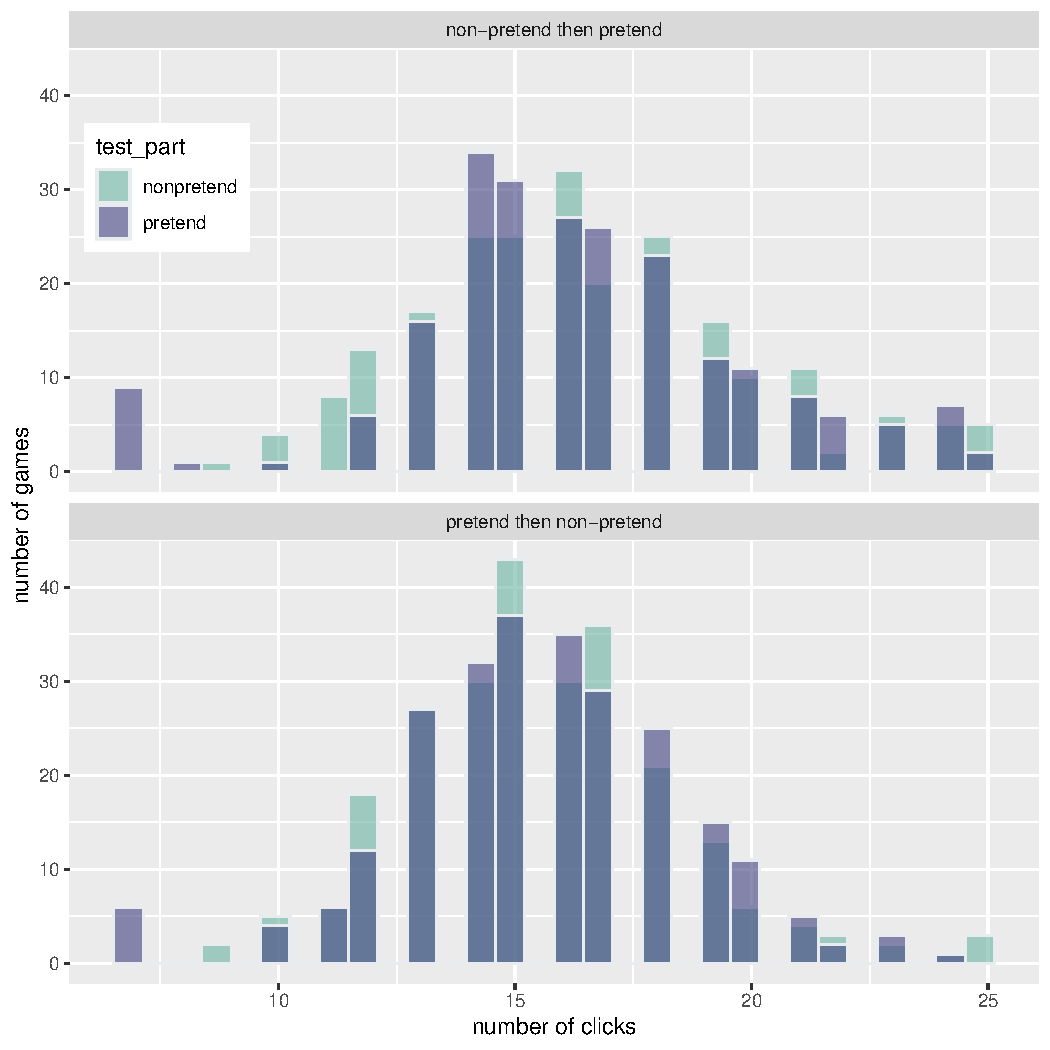
\includegraphics[width=1\linewidth]{figures/num_clicks} \caption{Number of clicks in pretend (purple) and non-pretend (green) games as a function of block order (pretend or non-pretend first).}\label{fig:num-clicks}
\end{figure}

\begin{verbatim}
## Warning: Removed 1 rows containing missing values (geom_point).
\end{verbatim}

\hypertarget{game-duration}{%
\subsection{Game duration}\label{game-duration}}

The median game duration was 20.21 seconds in the non-pretend condition and 28.56 seconds in the pretend condition. Pretend games were significantly longer than non-pretend games \(V = 3,783.00\), \(p < .001\). This difference showed a significant interaction with the order of conditions (\(F(1, 178) = 8.10\), \(\mathit{MSE} = 167.08\), \(p = .005\), \(\hat{\eta}^2_G = .044\)). Note that non-pretend blocks that were played after pretend blocks are not a good representation of players' natural playing behaviour. However, a difference in total game duration was observed also when comparing non-pretend games from non-pretend-first participants with pretend games from pretend-first participants (\(W = 577.00\), \(p < .001\)).

Overall, participants played 10 games on 9 different boards. 4 boards were used for non-pretend games, 4 for pretend games, and one board was used for both. When zeroing in on game durations for this common board, we observe a positive correlation across participants (and boards), such that participants that took longer in the non-pretend version also took longer in the pretend version (\(r = .51\), 95\% CI \([.34\), \(.65]\), \(t(89) = 5.61\), \(p < .001\)). This correlation held also when focusing on the non-pretend-first group (\(r = .56\), 95\% CI \([.31\), \(.73]\), \(t(41) = 4.29\), \(p < .001\)).

When taking the median game duration per board after excluding the non-pretend games of pretend-first participants, we see no correlation between pretend and non-pretend game durations across the nine boards (c(t = -2.62285551855581), c(df = 7), 0.0342666277642064, c(cor = -0.704027258410722), c(correlation = 0), two.sided, Pearson's product-moment correlation, E1.time\_per\_board\(pretend and E1.time_per_board\)nonpretend, c(-0.932261145377408, -0.0749484155796087)).

\begin{figure}[H]
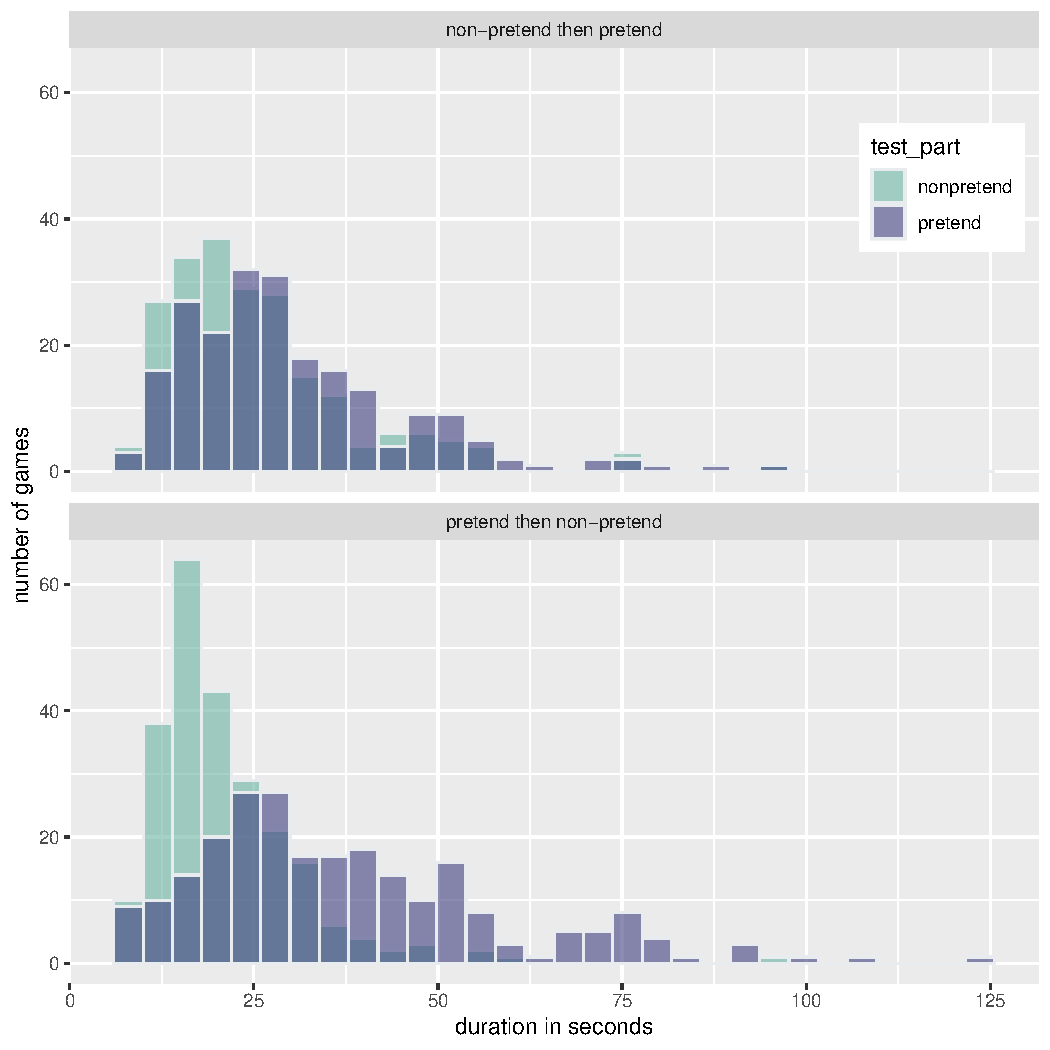
\includegraphics[width=1\linewidth]{figures/total_time} \caption{Total game duration in pretend (purple) and non-pretend (green) games as a function of block order (pretend or non-pretend first).}\label{fig:total-time}
\end{figure}

\hypertarget{reaction-times}{%
\subsection{Reaction times}\label{reaction-times}}

In non-pretend games, players were faster by 148 ms when hitting compared to missing a ship (\(V = 888.00\), \(p < .001\)). This effect was exaggerated in pretend games: players were faster by 384 ms in hits compared to misses (\(V = 1,119.00\), \(p < .001\)).

The opposite effect was observed for a hit on the previous click: players were slower by 130 ms after hitting a target (\(V = 171.00\), \(p < .001\)). Again, this effect was exaggerated in pretend games, where players were slower by 238 ms compared to misses (\(V = 255.00\), \(p < .001\)).

Finally, when sorting trials according to whether a ship was hit on the next trial, players were slower by 60 ms on the click preceding a hit (\(V = 670.00\), \(p = .017\)). This effect was not however preserved in pretend games (median difference: 30 ms; \(V = 550.00\), \(p = .703\)).

\hypertarget{discussion}{%
\section{Discussion}\label{discussion}}

\newpage

\hypertarget{references}{%
\section{References}\label{references}}

\begingroup
\setlength{\parindent}{-0.5in}
\setlength{\leftskip}{0.5in}

\hypertarget{refs}{}
\begin{CSLReferences}{0}{0}
\end{CSLReferences}

\endgroup


\end{document}
